\documentclass{scrbook}
\KOMAoptions{
	fontsize=11pt,
	paper=letter,
	paper=portrait,
	parskip=half,
	headings=big,
	chapterprefix=false,
	toc=listof,
	twoside=false,
	}
\usepackage[utf8]{inputenc}
\usepackage[T1]{fontenc}
\usepackage[english]{babel}
\usepackage[dvipsnames]{xcolor}
\usepackage[symbol]{footmisc}
\usepackage[margin=2.5cm]{geometry}
\usepackage{lmodern}
\usepackage{hyperref}
\usepackage{amsmath,amssymb,amsfonts,dsfont}
\usepackage{mathtools}
\usepackage[only, mapsfrom]{stmaryrd}
\usepackage{enumitem}
\setlist{nosep, noitemsep, label = (\textit{\roman*})}
\usepackage{todonotes}

\usepackage{tcolorbox}
\usepackage{amsthm}
\tcbuselibrary{many}

\newtcbtheorem[number within=chapter]{thm}{Theorem}{
	theorem style=plain apart,
	sharp corners,
	enhanced jigsaw,
	breakable,
	colback=NavyBlue!10,
	colbacktitle=NavyBlue!70!black,
	coltitle=White,
	boxrule=0pt,
	fonttitle=\sffamily\bfseries,
	description font=\normalfont\sffamily,
}{thm}

\newtcbtheorem[use counter from=thm]{lem}{Lemma}{
	theorem style=plain apart,
	sharp corners,
	enhanced jigsaw,
	breakable,
	colback=NavyBlue!10,
	colbacktitle=NavyBlue!70!black,
	coltitle=White,
	boxrule=0pt,
	fonttitle=\sffamily\bfseries,
	description font=\normalfont\sffamily,
}{lem}

\newtcbtheorem[use counter from=thm]{defn}{Definition}{
	theorem style=plain apart,
	sharp corners,
	enhanced jigsaw,
	breakable,
	colback=NavyBlue!10,
	colbacktitle=NavyBlue!70!black,
	coltitle=White,
	boxrule=0pt,
	fonttitle=\sffamily\bfseries,
	description font=\normalfont\sffamily,
}{defn}

\newtcbtheorem[use counter from=thm]{prop}{Proposition}{
	theorem style=plain apart,
	sharp corners,
	enhanced jigsaw,
	breakable,
	colback=NavyBlue!10,
	colbacktitle=NavyBlue!70!black,
	coltitle=White,
	boxrule=0pt,
	fonttitle=\sffamily\bfseries,
	description font=\normalfont\sffamily,
}{prop}

\newtcbtheorem[no counter]{que}{Question}{
	theorem style=plain apart,
	sharp corners,
	enhanced jigsaw,
	breakable,
	colback=NavyBlue!10,
	colbacktitle=NavyBlue!70!black,
	coltitle=White,
	boxrule=0pt,
	fonttitle=\sffamily\bfseries,
	description font=\normalfont\sffamily,
}{que}

\newtcbtheorem[no counter]{exmp}{Example}{
	theorem style=plain apart,
	sharp corners,
	enhanced jigsaw,
	breakable,
	colback=NavyBlue!10,
	colbacktitle=NavyBlue!70!black,
	coltitle=White,
	boxrule=0pt,
	fonttitle=\sffamily\bfseries,
	description font=\normalfont\sffamily,
}{exmp}

\newtcbtheorem[no counter]{dem}{Proof}{
	theorem style=plain,
	terminator sign={.},
	sharp corners,
	enhanced jigsaw,
	breakable,
	colframe=Black!20,
	colback=White,
	coltitle=Black,
	boxrule=2pt,
	fonttitle=\sffamily\itshape,
	description font=\normalfont\sffamily,
}{dem}

\newcommand{\lecture}[3]{
	%\newpage
	%\section{#3 (#2)}
	\todo[bordercolor = gray!30!white, backgroundcolor = gray!30!white, noline]{\scalebox{.65}{\sf #2}}
}

\usepackage{import}
\usepackage{pdfpages}
\usepackage{transparent}

\newcommand{\incfig}[2][1]{%
    \def\svgwidth{#1\columnwidth}
    \import{./figures/}{#2.pdf_tex}
}

\newcommand{\correct}[2]{\textcolor{Red!90!black}{\st{#1}} \textcolor{ForestGreen}{#2}}
\newcommand{\signexpl}[3]{\underset{\substack{\uparrow\\\mathrlap{\text{\hspace{#3}#2}}}}{#1}}


\title{Introduction to Syntax\\Lecture Notes}
\author{Guilherme Zeus Dantas e Moura\\\href{mailto:gdantasemo@haverford.edu}{\texttt{gdantasemo@haverford.edu}}}
\date{Haverford College --- Fall 2021\\Last updated: \today}

\begin{document}
	\maketitle

		This is Haverford College's undergraduate LING H113, instructed by Amanda Payne.
		All errors are my responsability.

		Use these notes only as a guide. There is a non-trivial chance that some things here are wrong or incomplete.
	

		\tableofcontents
		\newpage

	% start lectures
	\chapter{Introduction}
\lecture{1}{2021-08-30}{What is Syntax?}
\section{What do we study in syntax?}

Syntax is all about sentence \emph{structure.} Syntax is about \emph{form,} and semantics is about meaning. This has a few implications.

A \emph{sentence} is just a string of words. It doesn't necessarily have a meaning assigned to it. (A \emph{proposition} is a statement that has meaning and can be true or false.) We often represent sentences with written text for ease of analysis, but you can study the syntax of spoken or signed language.

\ex. It is raining today. \label{ex:1.1}

\ref{ex:1.1} is an example of a sentence in English. Most English speakers agree that \ref{ex:1.1} is \emph{grammatical}. That means it follows the rules of English syntax. We haven't talked about what exactly those rules are yet, but if you are an English speaker, you have some intuitions about what is grammatical and what is not. This data --- sentences and whether they are grammatical or not --- is our subject of study as syntacticians. Sometimes we can generate the data ourselves! But sometimes we can't, or shouldn't.

\ex. Íbsaan dháabata autóbusaa jíra. \label{ex:1.2}

\ref{ex:1.2} is a sentence from the language Oromo. It is also grammatical.

Some sentences are \emph{grammatical} --- they have a form that follows the rules --- but considered unacceptable. This is a major source of confusion for our data! Here are some such sentences:

\ex. That person is a real *****.
(Slurs are socially unacceptable, but typically grammatical.)

\ex. \# My toothbrush sneezed.
(Semantically unacceptable!)

Finally, grammar in linguistics is \emph{descriptive}, not \emph{prescriptive}. That means if a sentence would be naturally uttered by a speaker of a language, the sentence is considered grammatical for our data! This includes things like:

\ex. What should I talk about?
(Ending a sentence with a preposition happens all the time in speech.)

\ex. Who is this for?
(Using `who' where you might have been taught to use `whom'.)

Ungrammatical sentences are marked with *.
In-between or `marginally grammatical' sentences are marked with a ?.
Sentences that are semantically odd are marked with \#.

\ex. *Ungrammatical is sentence like this.

Grammaticality is not binary. Speakers of the same language can have different grammars, and therefore different judgments. Sometimes you might not even be sure if a given sentence is grammatical for you or not!

	\lecture{2}{2021-09-01}{The grammar}

\section{`The grammar'}

\emph{Grammar} in linguistics is what we call \emph{descriptive}, not \emph{prescriptive}. That means if a sentence would be naturally said by a speaker of a language, the sentence is considered \emph{grammatical} for our data. This includes:

\ex. What should I talk about? (Ending a sentence with a proposition happens all the time in speech.)

\ex. Who is this for? (Using `who' where you might have been taught to use `whom'.)

Judgments about grammaticality are usually innate. That means you can judge if a word or sentence ``sounds good'' in your language without any formal education or training.
You don't need to know how to read or write to have linguistic judgments.
In fact, very young children also have intuitions about language.

\subsection{The Wug Test}

\begin{figure}[htbp]
	\centering
	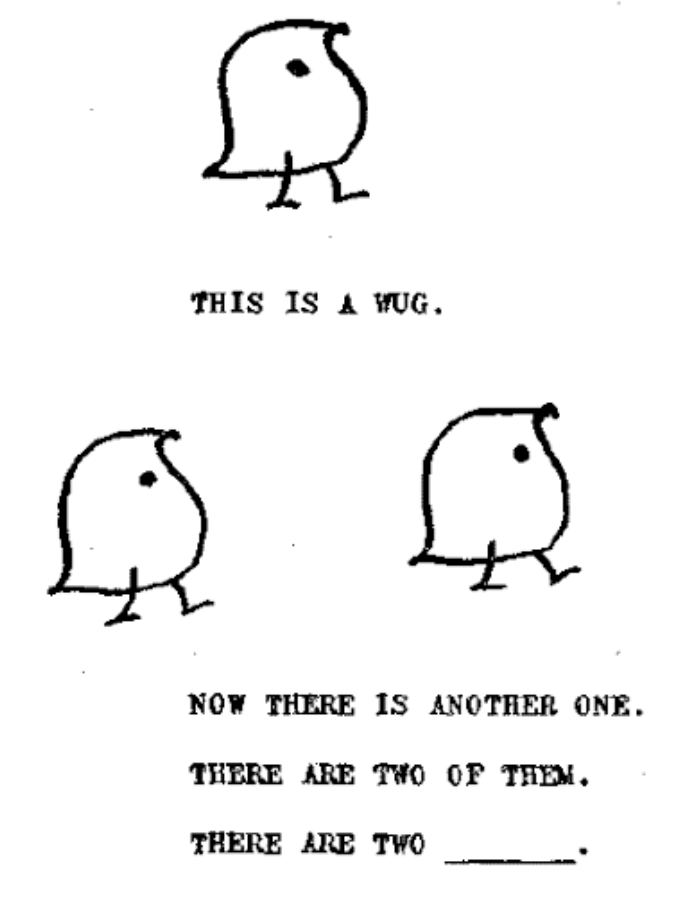
\includegraphics[width=.3\textwidth]{wug_test}
	\caption{The Wug Test (Berko, 1958)}
\end{figure}

The Wug test is checking the ability to generate a regular plural --- which is the suffix (-s) in English --- so this is in the realm of morphology and not necessarily syntax --- although there is a gray area between morphology and syntax, since how we define a single `word' is not super clear.

However, language users have intuitions in all areas of the grammar --- which will serve as a handy overview of generative linguistics.

\underline{Aside:} What is generative linguistics? This is a particular approach to studying language which assumes humans have a \emph{generative capacity}, i.e., the ability to generate linguistic forms, using some internal set of rules. This is often contrasted with \emph{funcionalist} approaches, which care more about the function of linguistic elements rather than the generative algorithm or set of rules used to produce them. These two approaches are actually compatible in most cases, but many colleges/linguists fall into one ``camp'' and might malign the other --- if they think about them at all. We will be looking at things through a generative lens in this class, but that doesn't mean it's the only way! 

\section{Areas of Linguistics}

\paragraph{Phonology.} The study of sound patters --- or patters in parameters of signs, for signed languages.

\ex. blick

\ex. ?bnick

\ex. *bfick

\paragraph{Morphology.} The study of word-internal structure --- like prefixes, suffixes, in-freakin'-fixes, etc. Not so different from syntax.

\ex. run

\ex. runs

\ex. run-(n)er

\ex. *run-s-er

\paragraph{Syntax.} The study of sentence structure --- like nouns, verbs, etc. More on this later.

\paragraph{Semantics.} The study of meaning as encoded in language.

\ex. I just stopped smoking. Now my lungs are feeling fresh.

\ex. I just stopped smoking. \#But in fact, I have never smoked.

\ex. \#This jar is green and not a jar.

\paragraph{Pragmatics.} The study of meaning in contex --- social context, language context, cultural context.

\ex. \emph{Don't tell your friends about your indigestion, ``how are you?'' is a greeting, not a question.}

\paragraph{Others.} Of course there are many other `named' areas of study in linguistics: socioling, anthroling, acquisition, compling, neuroling, psycholing, internet ling, phonetics, conversation analysis, philosophy of language, etc. --- but they are often overlapping/combined with the study of those various areas of the grammar listed above.

\chapter{Syntax}

Syntax is about how sentences are put together. In other to actually talk about the structure of a sentence, we need some categories, because there are too many words to list out individual rules. For example:

\begin{enumerate}[label = \textbullet, itemsep = 2pt]
	\item {[Noun Verb]} makes a fine sentence.
		
		\ex. Cats talk.

		\ex. Cats walk.

		\ex. Dogs talk.

		\ex. Dogs walk.

	\item But [Verb Noun] doesn't really (unless these are commands).

		\ex. *Talk cats.

		\ex. *Walk cats.

		\ex. *Talk dogs.

		\ex. *Walk dogs.

\end{enumerate}

So rather than listing \(\{\text{Cats}, \text{Dogs}, \dots\} + \{\text{Walk}, \text{Talk}, \dots\} = \text{English sentence}\), we can use the shorthands ``Noun'' and ``Verb''.






	\lecture{3}{2021-09-08}{Returning to our mini English grammar}

However, this rule \emph{overgenerates}, i.e., it produces sentences which are considered ungrammatical --- it produces too many sentences. For instance, \ref{ex:dogrun} and \ref{ex:dogsruns} are produced by this rule that we might want to exclude from our grammar.

\ex. *Dog run. \label{ex:dogrun}

\ex. *Dogs runs. \label{ex:dogsruns}

Of course, if we said our entire grammar was produced this rule, that would be a massive \emph{undergeneration}, since there are \emph{many} grammatical sentences of English which aren't generated by it, like \ref{ex:happydogsrun} and \ref{ex:dogsalwaysrun}.

\ex. Happy dogs run. \label{ex:happydogsrun}

\ex. Dogs always run. \label{ex:dogsalwaysrun}

\section{Syntactic primitives}

If we take the rule as our starting point, it's clear that we have two types of changes we need to make: we somehow need to introduce either more specific sub-types of nouns and verbs, to rule out things like \ref{ex:dogrun} and \ref{ex:dogsruns}, and we need to add more rules, to cover things like \ref{ex:happydogsrun} and \ref{ex:dogsalwaysrun}. Then, given more data, we might need to refine those new rules, too. This is a lot of what syntax is: coming up with rules, looking at data to see if the rules generate the data, and if not, changing the rules and starting again! In order to come up with these rules, we need some \emph{syntactic primitives}: basic categories of words that we can all agree on. So let's try it.

Now, upon combining our lists, we've probably got a lot of familiar terms like Nouns, Verbs, Adjectives, Adverbs, Prepositions, Determiners --- this is a solid foundation! We use these terms in syntax often, as they are extremely common across languages and can roughly be described in terms of their distribution in addition to their function. For instance, in English, \emph{nouns} are the types of things that can be pluralized, or the things that can follow a determiner. They often represent `people, places, and things' --- but not always. So rather than a meaning-based category, we want a distribution-based category.

You might have come up with a bunch of other terms that we may or may not end up using for our rules in this class --- things like conjunctions, particles, participles, or interjections. We will certainly talk about them as they become relevant to describing data as we see.

Finally, two noun-type things that we ought to consider specially: \emph{pronouns} and \emph{proper names}. Are these distinct syntactic categories from \emph{noun}? We have special names for them, but do they have an identical distribution to nouns like \emph{cat(s)}, \emph{dogs(s)}? What can we do with these?

	% end lectures
\end{document}
